\section{Ablations of PRS}
\label{ap:prs-ablations}
We perform an ablation study to evaluate the effect of the softness sampling design choice in PRS. Our default setting for \kernel{} is the combination of TRLOO, MRS, PR, and PRS, and we compare it to a variant, \kernel$_\text{w/o s in PRS}$, where kernels with $PR \geq \tau$ are kept directly, and kernels with $PR < \tau$ are discarded outright. In contrast, in the variant with softness, kernels with $PR \in [0.3, 0.4)$ are probabilistically retained, based on $PR$, $\tau$, and $s$. In this ablation, we set $\tau = 0.3$ as the fixed configuration.

As shown in Figure~\ref{fig:prs-softness}, \kernel{} outperforms the variant \texttt{w/o $s$ in PRS}. The variant still performs better and shows improved stability compared to the baseline \texttt{w/o PR \& PRS}. This ablation demonstrates that the softness sampling mechanism enhances the robustness of PRS, helping it balance correctness and meaningful speedup by selectively retaining relatively low-quality samples that might otherwise be discarded. This ability to retain such samples contributes to a more effective exploration-exploitation trade-off and facilitates more stable kernel generation over time.


\begin{figure*}[htbp]
  \centering
  % Row 1
  \begin{minipage}[t]{0.49\textwidth}
    \centering
    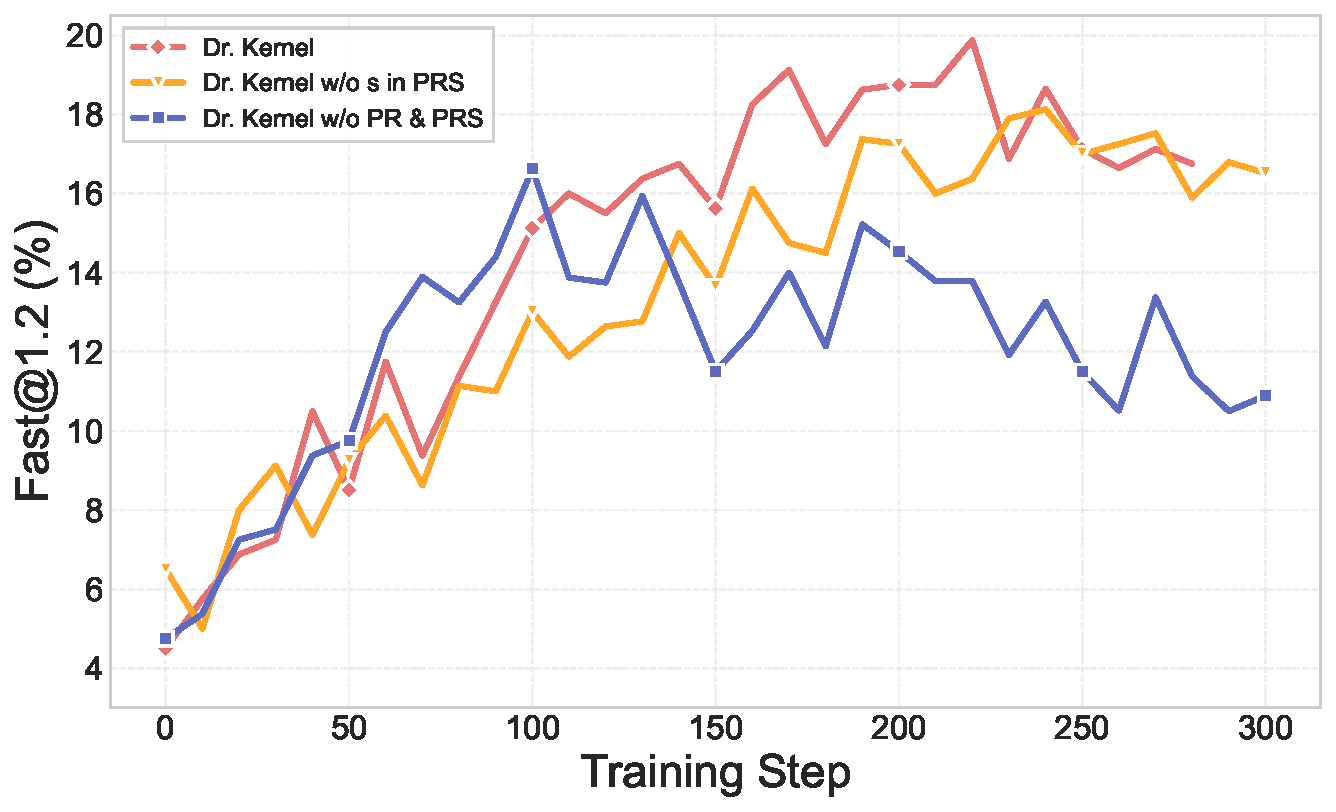
\includegraphics[width=\linewidth]{figures/prs-softness/prs_softness_comparison.pdf} % TODO
  \end{minipage}
  \caption{Comparison of \kernel{} with and without softness in PRS. \kernel{} outperforms the variant \texttt{w/o $s$ in PRS}, while both variants show better stability compared to the baseline \texttt{w/o PR \& PRS}.}
  \label{fig:prs-softness}
\end{figure*}